% This file was created by tikzplotlib v0.9.8.
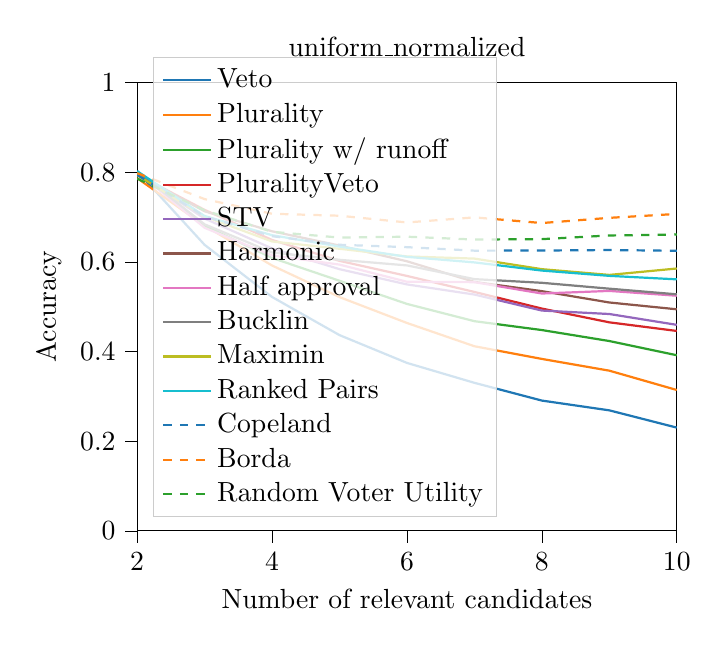
\begin{tikzpicture}

\definecolor{color0}{rgb}{0.12156862745098,0.466666666666667,0.705882352941177}
\definecolor{color1}{rgb}{1,0.498039215686275,0.0549019607843137}
\definecolor{color2}{rgb}{0.172549019607843,0.627450980392157,0.172549019607843}
\definecolor{color3}{rgb}{0.83921568627451,0.152941176470588,0.156862745098039}
\definecolor{color4}{rgb}{0.580392156862745,0.403921568627451,0.741176470588235}
\definecolor{color5}{rgb}{0.549019607843137,0.337254901960784,0.294117647058824}
\definecolor{color6}{rgb}{0.890196078431372,0.466666666666667,0.76078431372549}
\definecolor{color7}{rgb}{0.737254901960784,0.741176470588235,0.133333333333333}
\definecolor{color8}{rgb}{0.0901960784313725,0.745098039215686,0.811764705882353}

\begin{axis}[
legend cell align={left},
legend style={
  fill opacity=0.8,
  draw opacity=1,
  text opacity=1,
  at={(0.03,0.03)},
  anchor=south west,
  draw=white!80!black
},
tick align=outside,
tick pos=left,
title={uniform\_normalized},
x grid style={white!69.0196078431373!black},
xlabel={Number of relevant candidates},
xmin=2, xmax=10,
xtick style={color=black},
y grid style={white!69.0196078431373!black},
ylabel={Accuracy},
ymin=0, ymax=1,
ytick style={color=black}
]
\addplot [thick, color0]
table {%
2 0.8022
3 0.6379
4 0.5216
5 0.4365
6 0.3745
7 0.3301
8 0.2905
9 0.2687
10 0.2302
};
\addlegendentry{Veto}
\addplot [thick, color1]
table {%
2 0.7868
3 0.6804
4 0.5918
5 0.5213
6 0.4636
7 0.4117
8 0.3834
9 0.3572
10 0.3141
};
\addlegendentry{Plurality}
\addplot [thick, color2]
table {%
2 0.7998
3 0.6807
4 0.6087
5 0.5577
6 0.5061
7 0.4676
8 0.4478
9 0.4233
10 0.3916
};
\addlegendentry{Plurality w/ runoff}
\addplot [thick, color3]
table {%
2 0.7944
3 0.7159
4 0.6488
5 0.6021
6 0.5685
7 0.5328
8 0.4957
9 0.465
10 0.4458
};
\addlegendentry{PluralityVeto}
\addplot [thick, color4]
table {%
2 0.7965
3 0.6965
4 0.6299
5 0.5836
6 0.5496
7 0.527
8 0.4913
9 0.4836
10 0.4594
};
\addlegendentry{STV}
\addplot [thick, color5]
table {%
2 0.7947
3 0.7127
4 0.6681
5 0.6363
6 0.6012
7 0.5552
8 0.5346
9 0.5093
10 0.4941
};
\addlegendentry{Harmonic}
\addplot [thick, color6]
table {%
2 0.8008
3 0.6759
4 0.6142
5 0.5938
6 0.5555
7 0.5546
8 0.5293
9 0.5351
10 0.5244
};
\addlegendentry{Half approval}
\addplot [thick, white!49.8039215686275!black]
table {%
2 0.8013
3 0.6836
4 0.621
5 0.6045
6 0.592
7 0.5614
8 0.5532
9 0.5401
10 0.5275
};
\addlegendentry{Bucklin}
\addplot [thick, color7]
table {%
2 0.7933
3 0.7012
4 0.6454
5 0.6291
6 0.612
7 0.6072
8 0.5836
9 0.5708
10 0.5851
};
\addlegendentry{Maximin}
\addplot [thick, color8]
table {%
2 0.8023
3 0.7022
4 0.6594
5 0.634
6 0.6111
7 0.5987
8 0.5805
9 0.5687
10 0.5609
};
\addlegendentry{Ranked Pairs}
\addplot [thick, color0, dashed]
table {%
2 0.7939
3 0.7013
4 0.6572
5 0.638
6 0.6327
7 0.6249
8 0.6252
9 0.6263
10 0.6246
};
\addlegendentry{Copeland}
\addplot [thick, color1, dashed]
table {%
2 0.7978
3 0.7399
4 0.7072
5 0.7028
6 0.6878
7 0.6991
8 0.6865
9 0.6981
10 0.7068
};
\addlegendentry{Borda}
\addplot [thick, color2, dashed]
table {%
2 0.7856
3 0.715
4 0.6669
5 0.6541
6 0.656
7 0.6497
8 0.6506
9 0.6588
10 0.6608
};
\addlegendentry{Random Voter Utility}
\end{axis}

\end{tikzpicture}
